\documentclass[12pt]{report} % Increased the font size to 12pt
\usepackage{epigraph}
\usepackage{geometry}

% Optional: customize the style of epigraphs
\setlength{\epigraphwidth}{0.5\textwidth} % Adjust the width of the epigraph
\renewcommand{\epigraphflush}{flushright} % Align the epigraph to the right
\renewcommand{\epigraphrule}{0pt} % No horizontal rule
\usepackage[most]{tcolorbox}
\usepackage{amsmath, amssymb, amsthm}
\usepackage{graphicx}
\usepackage[utf8]{inputenc}
\usepackage{hyperref} % Added for hyperlinks
\usepackage{listings} % Added for code listings
\usepackage{color}    % Added for color definitions
\usepackage[super]{nth}
\usepackage{fancyhdr}
\usepackage{tikz}
\usepackage{cite}
\usetikzlibrary{shapes.geometric, arrows, positioning}

\tikzstyle{startstop} = [rectangle, rounded corners, text centered, draw=black, fill=red!30]
\tikzstyle{io} = [trapezium, trapezium left angle=70, trapezium right angle=110, text centered, draw=black, fill=blue!30]
\tikzstyle{process} = [rectangle, text centered, draw=black, fill=orange!30]
\tikzstyle{decision} = [diamond, text centered, draw=black, fill=green!30]
\tikzstyle{arrow} = [thick,->,>=stealth]

% Define the header and footer for general pages
\pagestyle{fancy}
\fancyhf{} % Clear all header and footer fields
\fancyhead{} % Initially, the header is empty
\fancyfoot[C]{\thepage} % Page number at the center of the footer
\renewcommand{\headrulewidth}{0pt} % No header line on the first page of chapters
\renewcommand{\footrulewidth}{0pt} % No footer line

% Define the plain page style for chapter starting pages
\fancypagestyle{plain}{%
  \fancyhf{} % Clear all header and footer fields
  \fancyfoot[C]{\thepage} % Page number at the center of the footer
  \renewcommand{\headrulewidth}{0pt} % No header line
}

% Apply the 'fancy' style to subsequent pages in a chapter
\renewcommand{\chaptermark}[1]{%
  \markboth{\MakeUppercase{#1}}{}%
}

% Redefine the 'plain' style for the first page of chapters
\fancypagestyle{plain}{%
  \fancyhf{}%
  \fancyfoot[C]{\thepage}%
  \renewcommand{\headrulewidth}{0pt}%
}

% Header settings for normal pages (not the first page of a chapter)
\fancyhead[L]{\slshape \nouppercase{\leftmark}} % Chapter title in the header
\renewcommand{\headrulewidth}{0.4pt} % Header line width on normal pages

\setlength{\headheight}{14.49998pt}
\addtolength{\topmargin}{-2.49998pt}
% Define colors for code listings
\definecolor{codegreen}{rgb}{0,0.6,0}
\definecolor{codegray}{rgb}{0.5,0.5,0.5}
\definecolor{codepurple}{rgb}{0.58,0,0.82}
\definecolor{backcolour}{rgb}{0.95,0.95,0.92}

% Setup for code listings
\lstdefinestyle{mystyle}{
    backgroundcolor=\color{backcolour},
    commentstyle=\color{codegreen},
    keywordstyle=\color{magenta},
    numberstyle=\tiny\color{codegray},
    stringstyle=\color{codepurple},
    basicstyle=\ttfamily\footnotesize,
    breakatwhitespace=false,
    breaklines=true,
    captionpos=b,
    keepspaces=true,
    numbers=left,
    numbersep=5pt,
    showspaces=false,
    showstringspaces=false,
    showtabs=false,
    tabsize=2
}

\lstset{style=mystyle}

% Definition of the tcolorbox for definitions
\newtcolorbox{definitionbox}[1]{
  colback=red!5!white,
  colframe=red!75!black,
  colbacktitle=red!85!black,
  title=#1,
  fonttitle=\bfseries,
  enhanced,
}

% Definition of the tcolorbox for remarks
\newtcolorbox{remarkbox}[1]{
  colback=blue!5!white,     % Light blue background
  colframe=blue!75!black,   % Darker blue frame
  colbacktitle=blue!85!black, % Even darker blue for the title background
  title=#1,            % Title text for remark box
  fonttitle=\bfseries,      % Bold title font
  enhanced,
}

% Definition of the tcolorbox for examples
\newtcolorbox{examplebox}[1]{
  colback=green!5!white,    % Light green background
  colframe=green!75!black,   % Darker green frame
  colbacktitle=green!85!black,  % Even darker green for the title background
  title=#1,         % Title text for example box
  fonttitle=\bfseries,    % Bold title font
  enhanced,
}

% Definitions and examples will be put in these environments
\newenvironment{definition}
    {\begin{definitionbox}}
    {\end{definitionbox}}

\newenvironment{example}
    {\begin{examplebox}}
    {\end{examplebox}}

\geometry{top=1.5in} % Adjust the value as needed
% ----------------------------------------------------------------



\begin{document}

\begin{titlepage}
  \centering
  \vspace*{2cm}
  {\LARGE\bfseries Report for C1 Research Computing Coursework\par}
  \vspace{1cm}
  {\Large\itshape\ CRSiD:\ tmb76\par}
  \vspace{1cm}
  {\Large\itshape\ University of Cambridge\par}
  \vfill
  {\large\today\par}
\end{titlepage}

\tableofcontents

\newpage
\vspace*{13\baselineskip}
\section*{Introduction}

In this report, an overview of the developping process of a python sudoku solver is given. The aim is to detail the software development of the solver, delving into the experimentation as well as how the code was improved, beyond it functioning as intended.

\chapter{Solving Algorithm and Prototyping}

\section{Solving a Sudoku Puzzle}

When solving a sudoku using brain-power, one has multiple techniques they can use. Most simple is to go through each cell, and using the sudoku constraints, eliminate impossible value, and hopefully be left with one. Relatively easy sudokus can be solved in part using this method. This can be referred to as the candidate-checking method\cite{cornell_sudoku}.
However, there usually comes a point where that process is no longer sufficient. From there, a good option is to mark up the possible values of each cell, and then spend a varying amount of time finding impossibilities for certain values by picturing future scenarios, similar to chess\cite{cornell_sudoku}.

\newpage
\section{Backtracking Algorithm}

A backtracking algorithm is the brute-force use of that latter method\cite{cornell_sudoku}.

\begin{definitionbox}{Naïve Backtracking Algorithm for a 9$\times$9 Sudoku}

  \begin{enumerate}
    \item Go through each cell (in a chosen order).
    \item In the current cell, enumerate from 1 to 9, until:
    \subitem{a.} A value is found that is valid.
    \subitem{b.} 9 is reached, and no valid value was found.
    \item In case of 2.a., go to the next cell and start again from Step 2.
    \item In case of 2.b., go back to the previous cell and, following from Step 2., try the next value.
  \end{enumerate}

\end{definitionbox}

\vspace*{1\baselineskip}
It is a rather simple algorithm to understand. It offers the guarantee of finding a solution, if one exists, eventually. It will even solve an empty grid though only finding one of the $6 \times 10^{21}$ possible solutions\cite{cornell_sudoku3}.
It is a brute-force algorithm, simply iterating through all possible combinations of values, until it finds one that is valid. On average, its speed depends on the number of empty cells, and the number of possible values for those cells, but can be sometimes very slow (see sec. 2.1.3). Additionaly, this naïve version, tests all values from 1 to 9. The cost of the algorithm is then at most $\mathcal{O}(9^{N_{empty cells}})$, where $N_{empty cells}$ is the number of empty cells in the sudoku.

\section{Modified Backtracking Algorithm}

The algorithm could take note of what values are possible for each cell, ahead of iterating through the sudoku. This would reduce the number of operations overall, coding wise.
From the candidate checking method, ``obvious'' values can be identified and filled in. Since possible values for each cell have to be marked up to do so. A modified backtracking algorithm that combines the both approaches can therefore be used, reducing the overall complexity of the algorithm to a maximum of $\mathcal{O}(N_{v}^{N_{empty cells}})$, where $N_{v}$ is the number of possible value for each cell, and $N_{v}\leq 9$.

\begin{definitionbox}{Modified Backtracking Algorithm with candidate checking for a 9$\times$9 Sudoku}

  \begin{enumerate}
    \item Markup the sudoku with the possible values for each cell.
    \item If the cell has only one possible value, fill it in.
    \item Go back to step 1 and repeat until no more cells can be filled in, i.e.\ the markup does not change.
    \item Start going through each cell (in a chosen order).
    \item In the current cell, enumerate through the possible values for that cell, until:
    \subitem{a.} A value is found that is valid.
    \subitem{b.} All values have been tried and none were valid.
    \item In case of 5.a., go to the next cell and start again from Step 5.
    \item In case of 5.b., go back to the previous cell and, following from Step 5., try the next value.
  \end{enumerate}

\end{definitionbox}

\newpage
\section{Prototyping}


The first idea of what the solver's code would look like was something like this:

\begin{figure}[bthp]
  \centering
  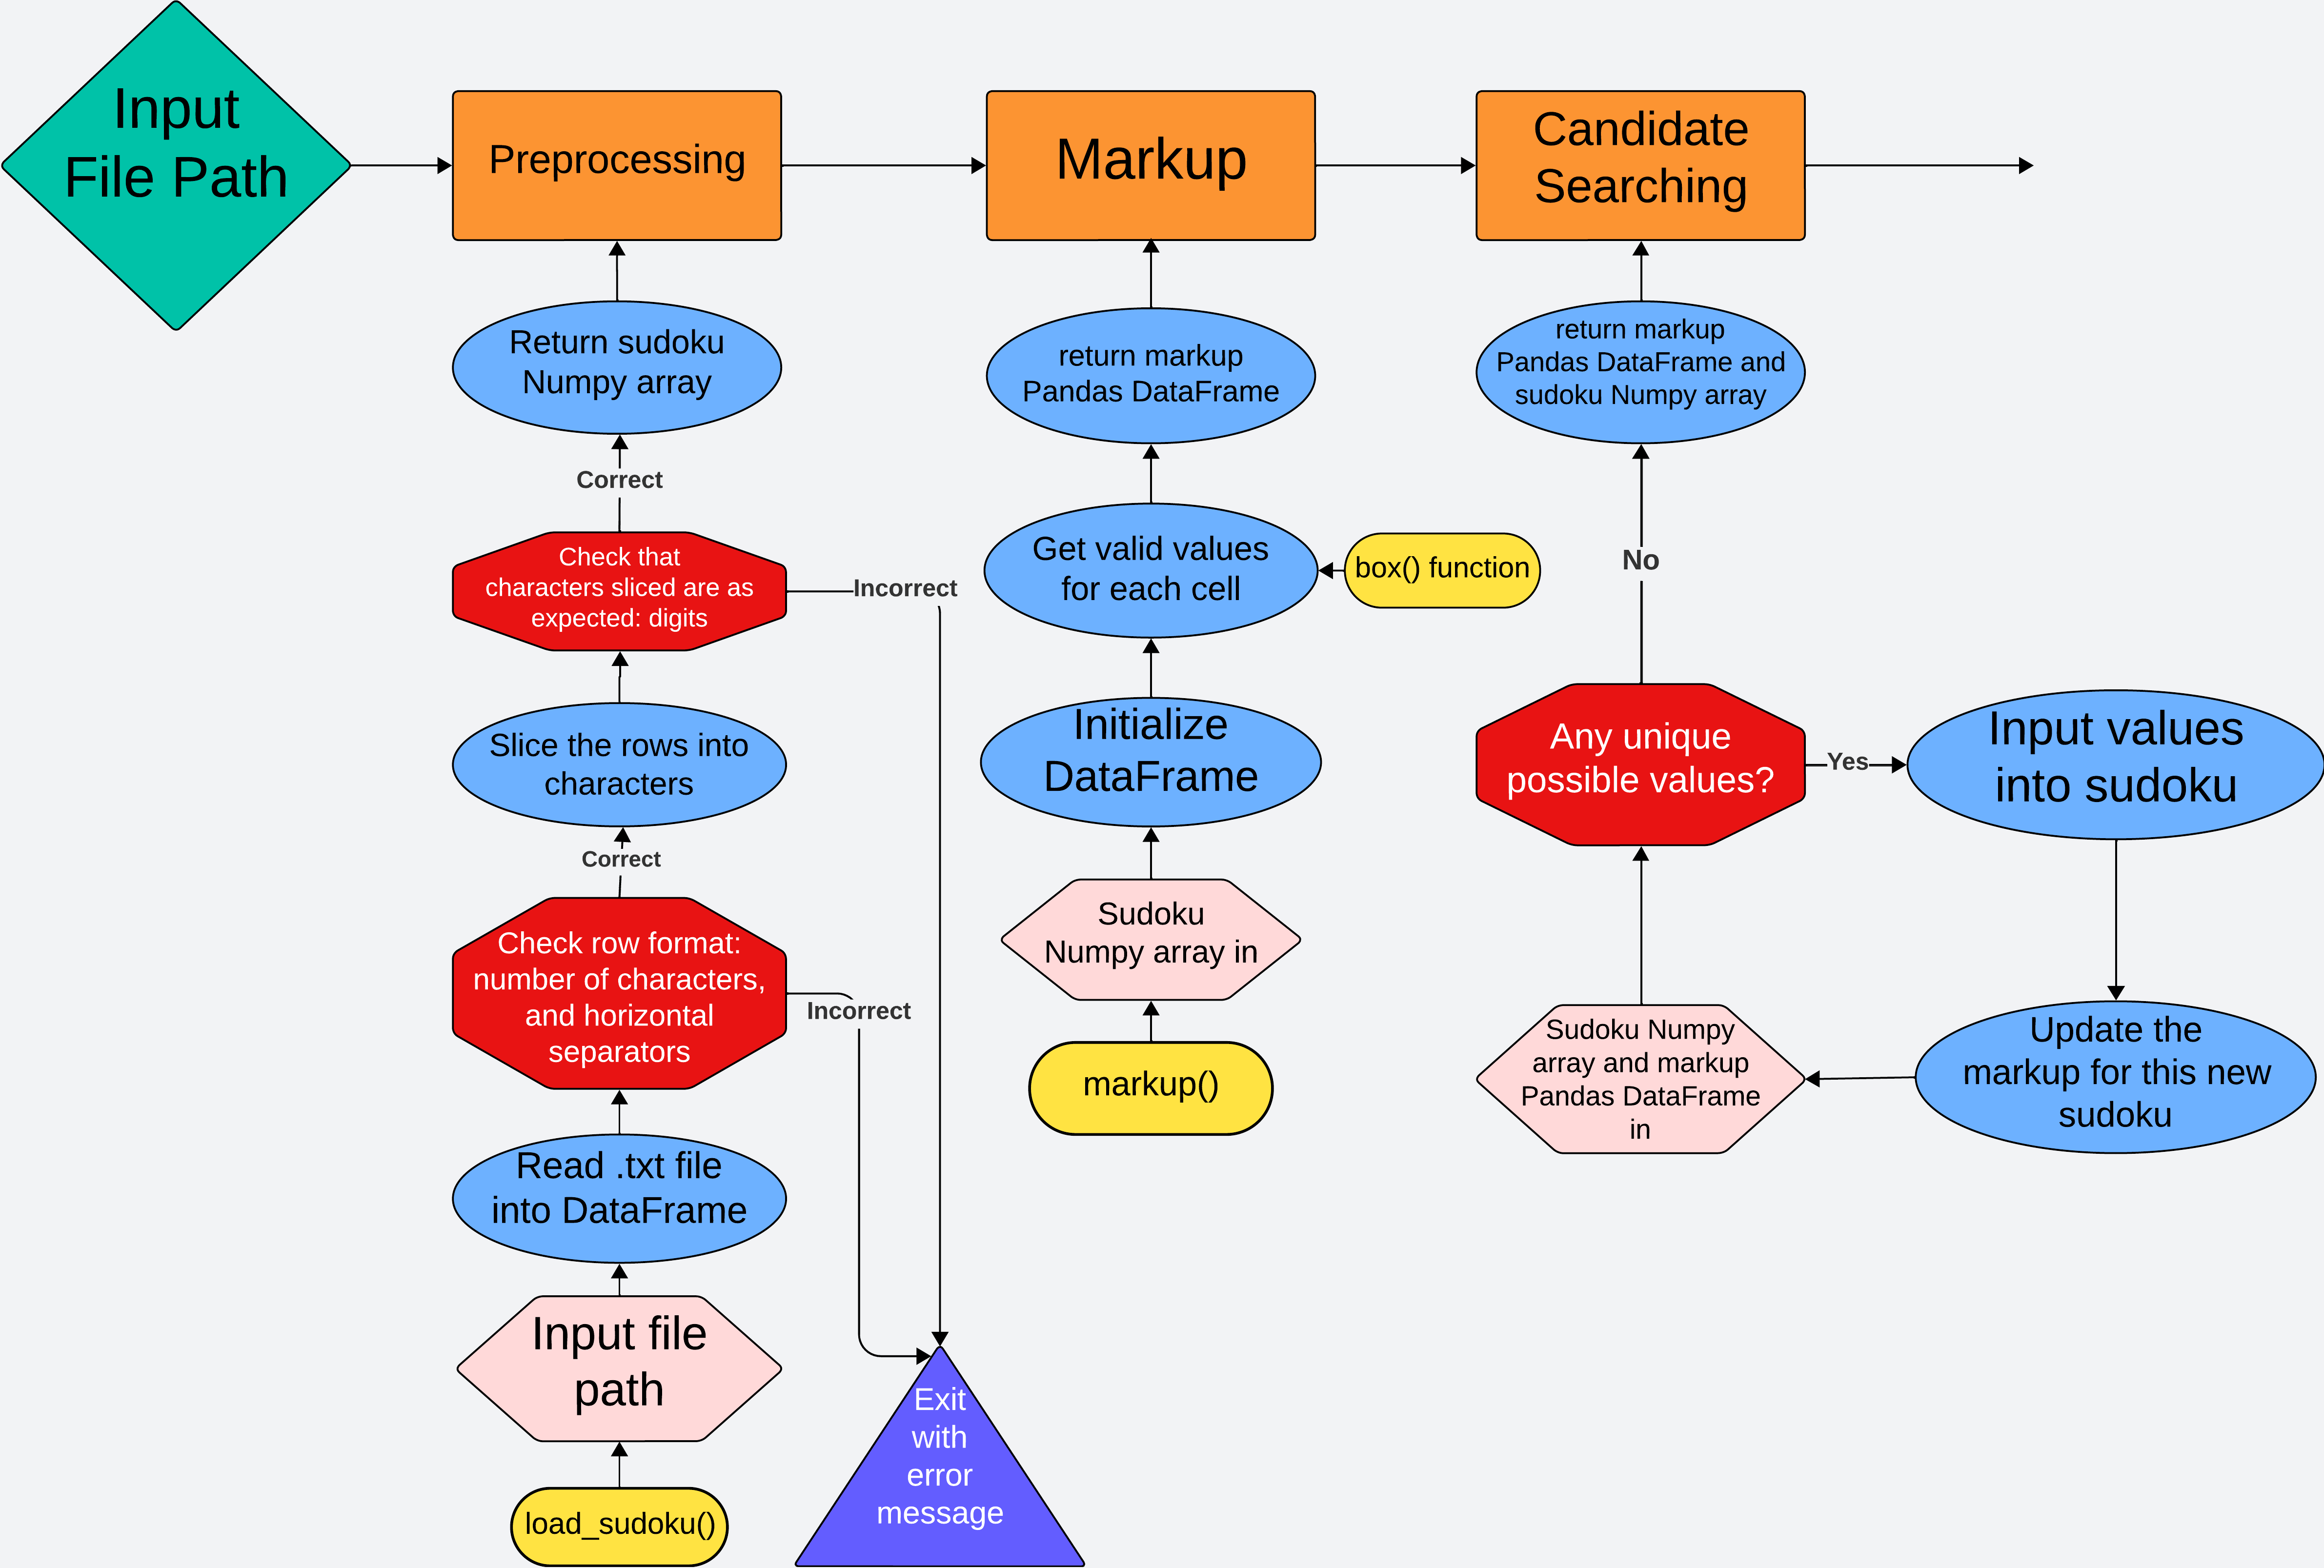
\includegraphics[width=\textwidth]{prototyping1.png}
  \caption{First prototyping of the solver}
\end{figure}

\begin{figure}[bthp]
  \centering
  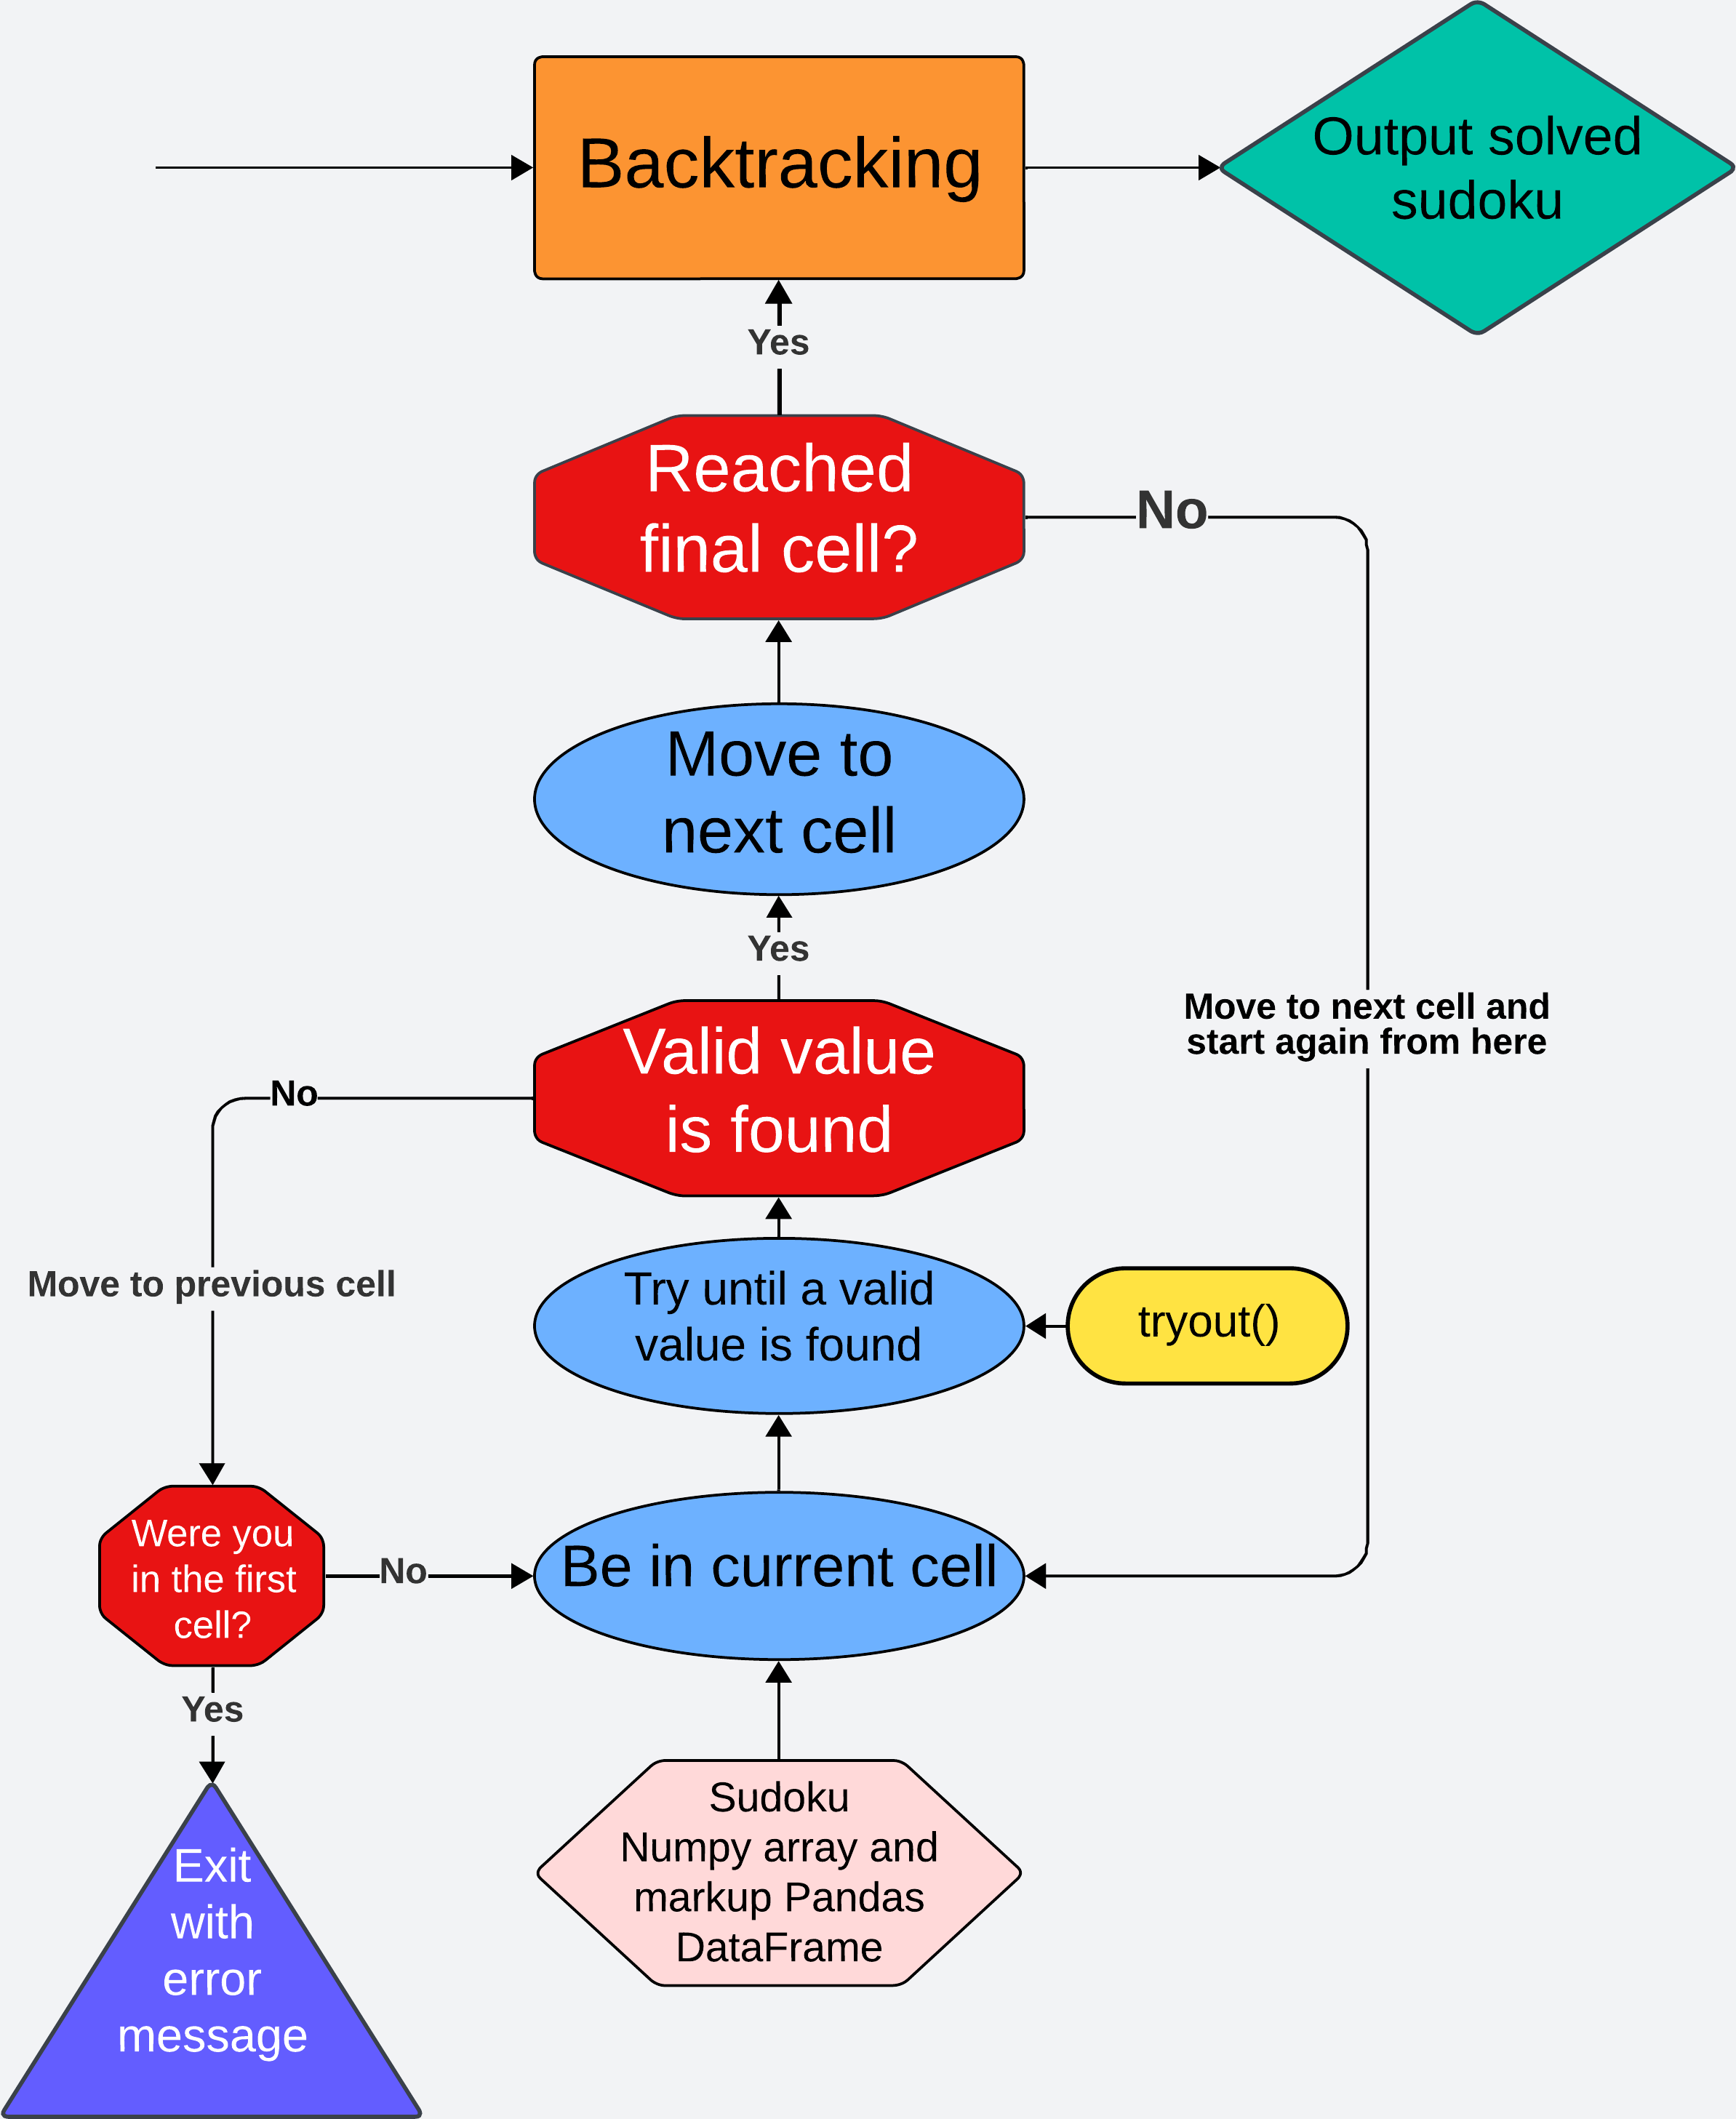
\includegraphics[width=0.8\textwidth]{prototyping1_next.png}
  \caption{First prototyping of the solver (continued)}
\end{figure}

\newpage
The solver would be runnable from the command line like so:

\begin{lstlisting}[language=bash]
  python solve_sudoku.py parameter.ini
\end{lstlisting}

Where the \texttt{parameter.ini} file would contain groups of paths to sudokus. Which parameters to use would be specified in the main \texttt{solve\_sudoku.py} file. The sudokus must be in a \texttt{.txt} file, with the following format, with 0's representing empty cells:

\vspace*{1\baselineskip}
\begin{lstlisting}[caption = {Sudoku input format example}]
020|000|000
000|083|400
090|000|000
---+---+---
000|800|000
600|009|000
000|000|093
---+---+---
000|100|000
000|054|000
070|000|000
\end{lstlisting}

\vspace*{1\baselineskip}
The \texttt{load\_sudoku()} function would read the sudoku from the file path and place the digits in a numpy array. Some checks would be done to ensure the sudoku \texttt{.txt} format is respected.
Following this preprocessing, the \texttt{markup()} function would look at each cell in the sudoku and, applying constraints, determine possible values. To check the 3$\times$3 box the cell is in, there would be a \texttt{box()} function to, given a sudoku, return all 3$\times$3 boxes of the sudoku. Finally, the markup values would be put in a Pandas DataFrame, as it allows for elements of different sizes.
Candidate searching would consist of inputing values in cells with unique possible values in the sudoku and updating the markup, until there are no unique possible values.
Then comes the backtracking part of the solver. Following the steps set out in the modified backtracking algorithm, the solver would go through each cell, and through the possible values. If it finds a valid one, it sets that value in the sudoku, and goes to the next still empty cell and starts trying out values again. If it doesn't find one there, it goes back to the previous cell and tries the next value. If it reaches the end of the possible values for the first cell (after reaching the last and backtracking all the way back to the first cell), the sudoku is thus unsolvable. The \texttt{tryout()} function would take in the cell location and the markup DataFrame, and return the first valid value it finds. It would be placed within a recursive loop that would go through each cell, and try out values until it finds a solution, or until it reaches the end of the possible values for the first cell. This would be handled by a \texttt{while} loop on the cell location.
Finally, the solved sudoku would be printed out to the command line.


\chapter{Development, Experimentation and Profiling}

\section{Development and experimentation}

\subsection{Markup and Box functions}


To avoid unnecessary memore use, the \texttt{box()} function was changed to take in the row and column number of the box wanted (e.g.\ the top right box would be box(1,3)), and return just that one. However, that meant finding out which box the cell was in, from its coordinates, before calling the \texttt{box()} function. With the \texttt{box()} function being called many times, it was better to take in the actual cell coordinates and return the box that cell is in.
In its first version, the \texttt{markup()} function would go through each unfilled cell and get the possible values for that cell, putting these in the markup dataframe, at the same coordinates. One problem was that the markup dataframe contained NaN values, for cells that were already filled. This could cause issues when comparing the markups. So, it was changed to input the cell's value in the dataframe. Suboptimally, updating the sudoku would mean re-inputing values that were already there.

\subsection{Candidate Checking}

To implement the candidate checking method, the markup function was put in a while loop whose condition was planned to be that there no longer were any unique possible values in the markup. But with the \texttt{markup()} function changes described above, it was changed to there being no difference between the updated markup and the previous one. In the case of an easy sudoku, this could be sufficient to solve it. So a break condition was added to the code before the backtracking, to return the sudoku if solved. Later, once the solver was working as intended, the \texttt{markup()} function was changed to allow for empty sudokus, giving a warning that there may be multiple solutions when the number of clues at the start of the sudoku is less than 17\cite{cornell_sudoku2}, rather than stopping the program.

\subsection{Backtracking}

The first attempt consisted of having an embedded \texttt{while} and \texttt{for} loop in which the \texttt{tryout()} function would be used. However, this would either need a complex set of loops, or somehow setting the number of embedded loops based on the number of empty cells. The main issue was how one would be able to go back to the previous iteration of the loop. Indeed, while there is a \texttt{continue} statement to skip to the next iteration, there isn't one to go back one\cite{stackoverflow_python_for_loop}. And though this cited stackoverflow post did provide an approach to have an iterator that could reverse one step, an other issue was the ability to keep track of the values already tried in the previous cell\cite{stackoverflow_python_for_loop}. Maybe by having a list to which tried values get added, but this seemed hard to follow, code-wise Thus, the method settled upon was to use a recursive function structure. The point of a recursive function is that it calls itself within its definition\cite{stackoverflow_recursion_python}:

\begin{lstlisting}[language=Python, caption = {Recursive function structure}]
  def recursive_function(args_1):
    if base_case:
      return something
    else:
      # do something
      recursive_function(args_2)
    # do something
    return something_else
\end{lstlisting}

In doing so, the function is called multiple times, at multiple ``recursive levels'' until a base case condition is fulfilled, a maximum number of recursive depth is reached\cite{stackoverflow_recursion_depth}, or something else depending on what the context and goal of the function is, which stops the recursion. The main benefit, is  that recursive levels are akin to embedded for loops, but without the worry of having to set the number of loops, so it is much neater when coded.
Backtracking for solving a sudoku falls under the category of exhaustive search where one tries all possible combinations. Following the Stanford lecture on Exhaustive search and backtracking[slides 13\-17]\cite{stanford_lecture}, this approach can be combined with returning booleans to handle whether to continue the recursion or end it. This gives the following structure:

\begin{examplebox}{Backtracking applied to sudoku}

    \begin{enumerate}
      \item \textbf{If} there are no more decisions to make:
      \subitem{a.}\textbf{Base case} If the sudoku is solved, i.e.\ we've reached the end of the sudoku still-empty cells, end the recursion. Return True.
      \subitem{b.}\textbf{Exhausted} If the sudoku is not solved, i.e.\ we've gone through every possibility, but there are no more possible values for the last cell, end the recursion. Return False.
      \item \textbf{Else:}
      \subitem{a.} \textbf{Choosing} Iterating over the still empty cells of the sudoku (markup cells with more than one possible value) using a recursive function. Choose a value from the markup cell's list, to which was applied the candidate checking method, to remove values that were no longer valid due to the filling up of the sudoku.
      \subitem{b.} \textbf{Exploring} Input that value in the sudoku, tracking our choice and move to the next cell, starting again at step 1.
      \subitem{c.} \textbf{Unchoosing} If going to the next cell, the valid values list is empty after running the validity check on it, reset the sudoku cell to 0 so that step 2.a.\ works properly, and go back to the previous cell and try the next value (i.e.\ go back to 2.).

    \end{enumerate}

\end{examplebox}


One issue with backtracking performance is it generally depends on the number of empty cells, and the number of possible values for each of those cells, but also the placement and values of the filled cells. In most cases, the algorithm only tries a tiny fraction of the possible combinations. But an ``anti-backtracking'' sudoku can easily be created or randomly found. The following sudoku is one such example, taking 1784.3329 seconds to solve\cite{stackoverflow_optimizing_backtracking_sudoku} (on a Macbook Air 2022, M2 chip, 8GB RAM):

\begin{lstlisting}[caption={anti\_backtracking.txt sudoku}]
900|800|000
000|000|500
000|000|000
---+---+---
020|010|003
010|000|060
000|400|070
---+---+---
708|600|000
000|030|100
400|000|200
\end{lstlisting}

But this is purely dependent on the order in which the algorithm iterates through the sudoku. Indeed, setting up a reverse order backtracking algorithm, this sudoku takes only 1.5 seconds to solve. This lead to also trying an ``ordered'' backtracking algorithm, choosing the cells with the least number of possible values first\cite{stackoverflow_optimizing_backtracking_sudoku}. To assess performance, a \texttt{perf\_timer.py} file was created, which used a large number of sudokus\cite{kaggle_sudoku_dataset}, and timed how long it took to solve them. Though the ``ordered'' method was expected to perform better, all 3 performed equally well.

\section{Profiling}


Having a working solver, \texttt{cProfile} was ran on our main \texttt{solve\_sudoku.py} file, we got the following output:


\begin{lstlisting}[language=Bash,caption={First profiling output, the right side describing what is running has been shortened for easier reading}, basicstyle=\tiny]
ncalls  tottime  percall  cumtime  percall filename:lineno(function)
    1    0.000    0.000    0.083    0.083 /src/solve_sudoku.py:25(solve_sudoku
    3    0.001    0.000    0.051    0.017 /src/solver_tools.py:54(markup)
  237    0.017    0.000    0.027    0.000 /src/solver_tools.py:94(<listcomp>)
318/1    0.001    0.000    0.019    0.019 /src/solver_tools.py:120(backtrack_alg)
  243    0.001    0.000    0.017    0.000 /pandas/core/series.py:1180(__setitem__)
  279    0.001    0.000    0.014    0.000 /pandas/core/series.py:1396(_maybe_update_cacher)
  317    0.011    0.000    0.014    0.000 /src/solver_tools.py:159(<listcomp>)
  243    0.001    0.000    0.011    0.000 /pandas/core/frame.py:4430(_maybe_cache_changed)
 3282    0.005    0.000    0.009    0.000 /src/preprocessing.py:89(box)
 3287    0.002    0.000    0.006    0.000 /numpy/core/fromnumeric.py:1768(ravel)
    3    0.002    0.001    0.006    0.002 /src/solver_tools.py:18(check_sudoku)
  279    0.000    0.000    0.006    0.000 /pandas/core/frame.py:3779(_ixs)
  643    0.002    0.000    0.006    0.000 /pandas/core/frame.py:3856(__getitem__)
  243    0.003    0.000    0.005    0.000 /pandas/core/internals/managers.py:1045(iset)
    6    0.000    0.000    0.005    0.001 /pandas/core/frame.py:668(__init__)
    5    0.000    0.000    0.004    0.001 /pandas/core/internals/construction.py:423(dict_to_mgr)
 3287    0.004    0.000    0.004    0.000 {built-in method numpy.asanyarray}
 3282    0.003    0.000    0.003    0.000 /src/preprocessing.py:128(<listcomp>)
  279    0.000    0.000    0.003    0.000 /pandas/core/frame.py:4387(_box_col_values)
  400    0.001    0.000    0.002    0.000 /pandas/core/series.py:1016(__getitem__)
  ....   .....    .....    .....    ..... mostly built-in functions of packages
\end{lstlisting}

A large amount of time was being spent on list comprehension lines used to get possible values, boxes, etc. This could be fixed by using sets. Sets have the advantage of only containing unique values\cite{freecodecamp_python_set_vs_list}. This means that originally, the code would search through the full row, column and box lists, with duplicates, and zeros. Whereas when using the union of the rows, columns, and boxes sets, we combine them in one set of at most 10 values. The time spent on these lines when running could thus be reduced significantly. The profiling output after this change was:

\begin{lstlisting}[language=Bash, caption={Profiling output after list comprehension improvements}, basicstyle=\tiny]
   ncalls  tottime  percall  cumtime  percall filename:lineno(function)
        1    0.000    0.000    0.047    0.047 /src/solve_sudoku.py:26(solve_sudoku)
        3    0.002    0.001    0.027    0.009 /src/solver_tools.py:56(markup)
      243    0.001    0.000    0.017    0.000 /pandas/core/series.py:1180(__setitem__)
      279    0.001    0.000    0.014    0.000 /pandas/core/series.py:1396(_maybe_update_cacher)
      243    0.001    0.000    0.011    0.000 /pandas/core/frame.py:4430(_maybe_cache_changed)
    318/1    0.003    0.000    0.010    0.010 /src/solver_tools.py:147(backtrack_alg)
      279    0.000    0.000    0.005    0.000 /pandas/core/frame.py:3779(_ixs)
      643    0.002    0.000    0.005    0.000 /pandas/core/frame.py:3856(__getitem__)
        3    0.002    0.001    0.005    0.002 /src/solver_tools.py:20(check_sudoku)
        6    0.000    0.000    0.005    0.001 /pandas/core/frame.py:668(__init__)
      243    0.003    0.000    0.005    0.000 /pandas/core/internals/managers.py:1045(iset)
        5    0.000    0.000    0.005    0.001 /pandas/core/internals/construction.py:423(dict_to_mgr)
      279    0.000    0.000    0.003    0.000 /pandas/core/frame.py:4387(_box_col_values)
      400    0.001    0.000    0.002    0.000 /pandas/core/series.py:1016(__getitem__)
     1283    0.002    0.000    0.002    0.000 /src/preprocessing.py:112(box)
     1288    0.001    0.000    0.002    0.000 /numpy/core/fromnumeric.py:1768(ravel)
      317    0.002    0.000    0.002    0.000 /src/solver_tools.py:191(<listcomp>)
5206/3341    0.001    0.000    0.002    0.000 {built-in method builtins.len}
        1    0.000    0.000    0.001    0.001 /pandas/core/frame.py:10039(map)
        1    0.000    0.000    0.001    0.001 /pandas/core/frame.py:9867(apply)
      243    0.000    0.000    0.001    0.000 /pandas/core/series.py:1270(_set_with_engine)
    ....     .....    .....    .....    ..... mostly built-in functions of packages

\end{lstlisting}

It can be seen the cumulative times are much lower, and the time spent on some lines was reduced by more than a factor of 10. This was all running for a near-empty sudoku that would make large use of the backtracking algorithm to solve:

\begin{lstlisting}[caption = {sudoku\_near\_empty.txt}]
000|000|000
001|000|200
000|000|000
---+---+---
000|000|000
000|000|000
000|000|000
---+---+---
000|000|000
000|000|000
000|000|000
\end{lstlisting}

Only timing the line where the \texttt{solve\_sudoku()} function is called, the improvement was from 0.049503 seconds to 0.020695 seconds after. One could see, however, that a large portion of the time is taken by pandas DataFrame functions (see Listing 2.4). Thus one could ask if the candidate checking method was actually slowing down the solver. Testing this using an easy sudoku which can be solved entirely by the candidate checking method:

\begin{lstlisting}[caption= {sudoku\_easy.txt}]
002|560|470
058|403|000
004|020|008
---+---+---
781|000|040
409|100|726
006|047|800
---+---+---
007|006|013
005|030|007
060|709|200
\end{lstlisting}
\newpage
The following profiling output was obtained:

\begin{lstlisting}[language=Bash, caption={Profiling output for easy sudoku},basicstyle=\tiny]
          ncalls  tottime  percall  cumtime  percall filename:lineno(function)
          1    0.001    0.001    0.161    0.161 /src/solve_sudoku.py:26(solve_sudoku)
         18    0.005    0.000    0.138    0.008 /src/solver_tools.py:56(markup)
       1458    0.004    0.000    0.098    0.000 /pandas/core/series.py:1180(__setitem__)
       1629    0.005    0.000    0.078    0.000 /pandas/core/series.py:1396(_maybe_update_cacher)
       1458    0.004    0.000    0.063    0.000 /pandas/core/frame.py:4430(_maybe_cache_changed)
       1620    0.003    0.000    0.031    0.000 /pandas/core/frame.py:3779(_ixs)
       1458    0.013    0.000    0.026    0.000 /pandas/core/internals/managers.py:1045(iset)
       2728    0.008    0.000    0.023    0.000 /pandas/core/frame.py:3856(__getitem__)
       1620    0.002    0.000    0.017    0.000 /pandas/core/frame.py:4387(_box_col_values)
         19    0.000    0.000    0.016    0.001 /pandas/core/frame.py:668(__init__)
         19    0.001    0.000    0.015    0.001 /pandas/core/internals/construction.py:423(dict_to_mgr)
26809/15959    0.005    0.000    0.009    0.000 {built-in method builtins.len}
       1620    0.001    0.000    0.008    0.000 /pandas/core/frame.py:656(_constructor_sliced_from_mgr)
       1458    0.001    0.000    0.008    0.000 /pandas/core/series.py:1270(_set_with_engine)
       1620    0.005    0.000    0.007    0.000 /pandas/core/internals/managers.py:991(iget)
       1458    0.002    0.000    0.007    0.000 /pandas/core/series.py:1385(_check_is_chained_assignment_possible)
       1270    0.002    0.000    0.007    0.000 /pandas/core/series.py:1016(__getitem__)
       2728    0.002    0.000    0.006    0.000 /pandas/core/frame.py:4405(_get_item_cache)
       1458    0.001    0.000    0.006    0.000 /pandas/core/internals/managers.py:1977(setitem_inplace)
       1639    0.004    0.000    0.005    0.000 /pandas/core/generic.py:6147(__finalize__)
       5456    0.004    0.000    0.005    0.000 /pandas/core/indexing.py:2678(check_dict_or_set_indexers)
47346/47327    0.004    0.000    0.005    0.000 {built-in method builtins.isinstance}
       4186    0.003    0.000    0.005    0.000 /pandas/core/indexes/range.py:394(__contains__)
          3    0.002    0.001    0.005    0.002 /src/solver_tools.py:20(check_sudoku)
       ....    .....    .....    .....    ..... mostly built-in functions of packages
\end{lstlisting}

Running the solver for this sudoku, it found a solution in 0.05651 seconds but did so much quicker in 0.00988 seconds when only getting the markup file once without updating it, and running backtracking from there. Unfortunately, this meant that conducting a candidate check to get rid of obvious values was actually not reducing the solving time overall. Using the \texttt{perf\_timer.py} file described in section 3.1.3., a comparison was made between average runtime for many sudokus, with and without the candidate checking method. The results showed almost a factor of 3 decrease in runtime when using backtracking only and marking up the sudoku just once (Backtracking only takes 0.0054 compared to 0.0167 seconds).

\subsection{Future improvements}

Unlike the assumption made in section 2.4., numpy arrays of 3 dimensions can contain lists of different sizes, so an improvement in memory use could be made by switching to numpy for the markups\cite{numpy_vs_pandas}.
In the interest of approaching sudokus with multiple solutions, a random backtracking order could be set up to shuffle the backtracking cells using \texttt{numpy.random.suffle()} on the backtrack cells list, this way obtaining many different solutions. Though it would run the risk of being slow, as we know the order of the cells has a large impact on the runtime.

\chapter{Validation, Unit Tests and CI set up}

\section{Validation and Unit Tests}

Most sudokus in the offered \texttt{sudokus/} directory were obtained from the sudoku app from sudoku.com\cite{sudoku_com} by EasyBrain. Thus, the solutions given by the solver were checked using these. More importantly, a \texttt{check\_sudoku()} function was written to check that the sudoku is at least valid. This means checking there are no duplicates in the rows, columns and boxes. It was used at different points in the solver, checking the sudoku is valid after loading, after candidate checking, and after backtracking. Particularly useful in the \texttt{perf\_timer.py} file, since the solutions are not returned, it checks that the solver did indeed find a valid solution. It takes an argument \texttt{final\_check} which, if set to True, will check there are no empty cells left.
Multiple error traps were set in the functions and main code. They include checks to ensure the format of the input sudoku is correct, and multiple checks to ensure the sudoku is valid at different points in the solver, and that it is not unsolvable. If any of these checks fail, the solver will stop and print an appropriate error message, with a traceback to the line where the error occured, or a warning.
Unit tests were also set up. They are mostly straightforward, and they check the functions return the expected outputs. They either check that the correct answer is given or, for a given ``bad'' input, that corresponding errors and warnings are raised.

\section{CI set up}

Continuous Integration of this project was set up using a \texttt{pre-commit-config.yaml} file. This sets up automatic checks on the code before every commit:

\begin{enumerate}
  \item \textbf{\texttt{check-yaml}} Checks that the \texttt{.yaml} files were not changed. This includes the \texttt{pre-commit-config.yaml} file itself.
  \item \textbf{\texttt{end-of-file-fixer}}, \textbf{\texttt{trailing-whitespace}}, \textbf{\texttt{mixed-line-ending}} Checks the end of the files are correct. This is to ensure that the files end with a new line, and that the line endings are consistent.
  \item \textbf{\texttt{debug-statements}} Checks that there are no debugging statements left in the code. This is to ensure that the code is clean and ready to be run.
  \item \textbf{\texttt{black}} Checks the format of the code, and reformats it if necessary. It is there to minimize the number of errors the next hook could find.
  \item \textbf{\texttt{flake8}} Checks the code for PEP8 compliance. It is there to ensure the code is clean and readable, following a set of standards. E.g. line length cannot exceed 79 characters (due to most code editors having set window widths\cite{pep8_}).
  \item \textbf{\texttt{pytest}} Runs all the files that fall under a certain naming convention (Here: \texttt{\^test//test\_.\*\.py}, i.e.\ all files in the \texttt{test/} directory that start with \texttt{test\_} and end with \texttt{.py}, to avoid an error with pytest catchin the \texttt{\_\_pycache\_\_} files in the \texttt{test/} directory).
\end{enumerate}

The code was also written with Doxygen compatible documentation, and accordingly, there was a \texttt{Doxyfile} created to generate the documentation. There should be a \texttt{html/} folder in the \texttt{docs/} directory, but Doxygen can be run to regenerate it if missing.


\chapter{Packaging and Usability}

\section{Packaging}

The structure of the project is as follows:


\begin{lstlisting}[caption={Directory Structure},basicstyle=\tiny]

  sudoku_solver/
  |-- docs/
  |   |-- Doxyfile
  |    -- html/
  |-- profiling/
  |   |-- perf_timer.py
  |   |-- profiling.py
  |    -- profile.txt
  |-- report/
  |   |-- refs.bib
  |   |-- report.pdf
  |    -- report.tex
  |-- src/
  |   |-- __init__.py
  |   |-- preprocessing.py
  |   |-- solver_tools.py
  |    -- solve_sudoku.py
  |-- sudokus/
  |   |-- anti_backtracking.txt
  |   |-- bad_format_sudoku.txt
  |   |-- dad_sudoku.txt
  |   |-- sudoku_easy.txt
  |   |-- sudoku_near_empty.txt
  |   |-- sudoku_test.txt
  |   |-- sudoku1.txt
  |    -- sudoku2.txt
  |-- test/
  |   |-- __init__.py
  |   |-- test_preproc.py
  |   |-- test_markup.py
  |   |-- test_backtrack.py
  |    -- test_check_sudoku.py
  |-- .gitignore
  |-- .pre-commit-config.yaml
  |-- Dockerfile
  |-- environment.yml
  |-- Instructions.md
  |-- LICENSE
   -- README.md

\end{lstlisting}

\section{Usability}

The repository comes with a Dockerfile which the user is encouraged to use. Once the image built and the container running (specific instructions can be found in the README), the main solver file \texttt{solve\_sudoku.py} can then be run from the command line using the following command:

\begin{lstlisting}[language=bash, caption={How to run the solver}]
  python -m src.solve_sudoku path/to/sudoku.txt 'backtracking_type' backtracking_only
\end{lstlisting}

The \texttt{-m} flag is used to run the file as a module, which is to deal with the relative imports in the code. The \texttt{path/to/sudoku.txt} is the path to the sudoku file, in the format specified in Listing 2.1. The \texttt{backtracking\_type} argument can either be \texttt{'forward'}, \texttt{'backward'}, or \texttt{'ordered'}. The \texttt{backtracking\_only} argument is a \texttt{Bool} value, and is used to set the solver to only use backtracking (\texttt{True}) or also use the candidate checking method (\texttt{False}). The solver will print the solved sudoku to the command line, and also write a \texttt{.txt} file with the same name as the input sudoku file, in a \texttt{sudoku\_solution/} directory, which will get created if it doesn't exist yet.

For the \texttt{perf\_timer.py} and \texttt{profiling.py} files, the user can run them from the command line using the following commands:

\begin{lstlisting}[language=bash, caption={How to run the profiling and timing files}]
  python -m profiling.perf_timer path/to/sudokus.csv backtracking_only
  python -m profiling.profiling path/to/sudoku.txt 'backtracking_type' backtracking_only
\end{lstlisting}

For the \texttt{perf\_timer.py} file, the sudokus.csv can be obtained from this kaggle website\cite{kaggle_sudoku_dataset}. One can decide to only take a subset of the available sudokus. For the timing results in Chapter 3, around 2000 sudokus were used.


\chapter{Summary}

Thus, our sudoku solver now works as intended. It can solve any sudoku, eventually, though giving at most 3 solutions to sudokus with a large number of solutions.

\bibliographystyle{plain}
\bibliography{refs.bib}

\end{document}
